
\documentclass[10 pt,usenames,dvipsnames, oneside]{article}
\usepackage{../../../modelo-ensino-medio}


\begin{document}

\begin{center}
  \begin{minipage}[l]{3cm}
\includegraphics[width=2cm]{logo}    
\end{minipage}\hfill
\begin{minipage}[r]{.8\textwidth}
 {\Large \scshape Atividade: As imagens}  
\end{minipage}
\end{center}
\vspace{.2cm}

\ifdefined\prof
\begin{objetivos}
\item \textbf{LAF3} Calcular e interpretar a taxa de variação média de uma função em um intervalo dado, tanto algebricamente quanto a partir de dados gráficos ou de uma tabela, identificando tendências de crescimento e decrescimento.
\end{objetivos} 

\begin{goals}
\begin{enumerate}

\item [OE1] Calcular imagens de alguns pontos sendo conhecidas as taxas de variação médias em intervalos do domínio.

\item [OE2] Relacionar a disposição dos pontos no gráfico com a variação da taxa de variação média.

\end{enumerate}

\tcblower

\begin{itemize}

\item A principal atenção na hora de fazer as contas deve estar nos intervalos em que estão
definidas as taxas médias.
\item Ao finalizar a atividade, estimule que os estudantes façam conjecturas sobre a variação
da taxa e a forma do gráfico. Por exemplo, “o que ocorre quando a taxa é igual a zero?”,
“se for constante e positiva?”, “constante e negativa?”, “qual a forma do gráfico quando
a taxa de variação é crescente?", “e decrescente?” etc.
\item Como extensão, proponha que os estudantes investiguem que taxas médias gerariam
outras formas de gráficos; desafie-os a conjecturar ou pelo menos a dar exemplos de
taxas que correspondam às formas abaixo,

\begin{multicols}{5}
\begin{center}

\begin{tikzpicture}

\draw (-1,0) -- (1,0);
\draw (0,-1) -- (0,1);

\draw [domain=-1:1, session3, thick] plot (\x,{\x^3});
\end{tikzpicture}

\begin{tikzpicture}

\draw (-1,0) -- (1,0);
\draw (0,-1) -- (0,1);

\draw [domain=-1:1, session3, thick] plot (\x,{-\x^3});
\end{tikzpicture}

\begin{tikzpicture}

\draw (-1,0) -- (1,0);
\draw (0,-1) -- (0,1);

\draw [domain=-1:1, session3, thick] plot (\x,{-(\x)^2});
\end{tikzpicture}

\begin{tikzpicture}

\draw (-1,0) -- (1,0);
\draw (0,-1) -- (0,1);

\draw [domain=-1:1, session3, thick] plot (\x,{(\x)^2});
\end{tikzpicture}

\begin{tikzpicture}

\draw (-1,0) -- (1,0);
\draw (0,-1) -- (0,1);

\draw [domain=0:1, session3, thick] plot (\x,{(\x)^2-2*(\x)});

\draw [domain=0:-1, session3, thick] plot (\x,{-(\x)^2-2*(\x)});

\end{tikzpicture}

\end{center}
\end{multicols}
\end{itemize}
\end{goals}

\bigskip
\begin{center}
{\large \scshape Atividade}
\end{center}
\fi

Nas tabelas abaixo encontram-se as taxas de variação médias de funções e os intervalos correspondentes. Complete-as com os valores da função e em seguida represente os pontos no sistema de coordenadas
\begin{equation*}
\frac{\Delta y}{\Delta x}=\frac{f(b)-f(a)}{b-a}
\end{equation*}
\ifdefined\prof
\clearpage
\fi
\begin{enumerate}
\item \phantom{coisa}

  \begin{minipage}{.4\textwidth}
 \begin{table}[H]
    \setlength\tabcolsep{2.5pt}
\begin{tabu} to .4\textwidth{|c|c|c|}
  \hline
  \thead
  $\bm{[a,b]}$ & $\bm{f(0) = 1}$ & $\bm{\Delta y/\Delta x}$ \\
  \hline
  $[0,1]$ & $f(1) = \phantom{1000} $ & 2 \\
  \hline
  $[1,2]$ & $f(2) = \phantom{1000} $ & 2 \\
  \hline
  $[2,3]$ & $f(3) = \phantom{1000} $ & 2 \\
  \hline
  $[3,4]$ & $f(4) = \phantom{1000} $ & 2 \\  
  \hline
\end{tabu}
\end{table}
\end{minipage}\hfill
\begin{minipage}{.4\textwidth}
  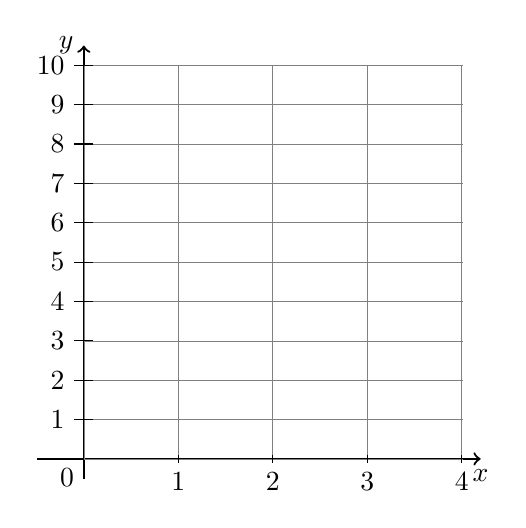
\begin{tikzpicture}[yscale=.5,xscale=1.2]
    \draw [->, thick] (0,-.5) -- (0,10.5) node[left] {$y$};
    \draw [->, thick] (-.5,0) -- (4.2,0) node[below] {$x$};
    \draw[help lines, gray] (0,0) grid (4.01,10.01);
    \foreach \x in {1,...,4} \draw (\x,.1)  -- (\x,-.1)  node[below] {\x};
    \foreach \y in {1,...,10} \draw (.1,\y) -- (-.1,\y) node[left] {\y};        
\node[below left] at (0,0) {0};
  \end{tikzpicture}
  \end{minipage}
\item  \phantom{coisa}

  \begin{minipage}{.4\textwidth}
   \begin{table}[H]
   \setlength\tabulinesep{1mm}
   \setlength\tabcolsep{2.5pt}
\begin{tabu} to .4\textwidth{|m{.3\textwidth}|m{.35\textwidth}|c|}
  \hline
  \thead
  $\bm{[a,b]}$ & $\bm{f(0) = 10}$ & $\bm{\Delta y/\Delta x}$ \\
  \hline
  $[0,\frac{1}{2}]$ & $f(1/2) = $ & -2 \\
  \hline
  $[\frac{1}{2},1]$ & $f(1) = $  & -2 \\
  \hline
  $[1,\frac{3}{2}]$ & $f(3/2) =$  &-2 \\
  \hline
  $[\frac{3}{2},2]$ & $f(2) = $  &-2 \\
  \hline
  $[2,\frac{5}{2}]$ & $f(5/2) =$  &-2 \\
  \hline
  $[\frac{5}{2},3]$ & $f(3) = $  &-2 \\
  \hline
  $[3,\frac{7}{2}]$ & $f(7/2) =$   &-2 \\
  \hline
  $[\frac{7}{2},4]$ & $f(4) =$   &-2 \\
  \hline
\end{tabu}
\end{table}
\end{minipage}\hfill
\begin{minipage}{.4\textwidth}
  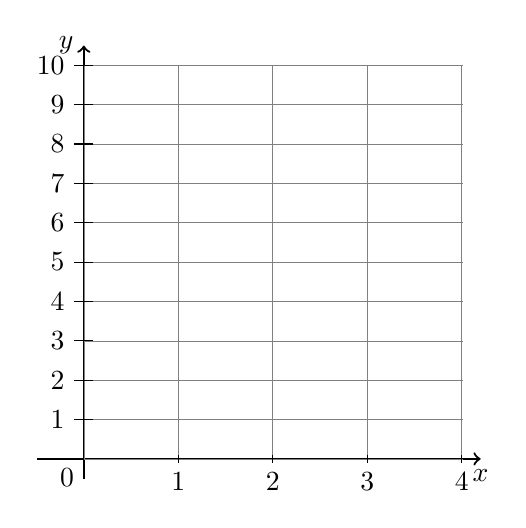
\begin{tikzpicture}[yscale=.5,xscale=1.2]
    \draw [->, thick] (0,-.5) -- (0,10.5) node[left] {$y$};
    \draw [->, thick] (-.5,0) -- (4.2,0) node[below] {$x$};
    \draw[help lines, gray] (0,0) grid (4.01,10.01);
    \foreach \x in {1,...,4} \draw (\x,.1)  -- (\x,-.1)  node[below] {\x};
    \foreach \y in {1,...,10} \draw (.1,\y) -- (-.1,\y) node[left] {\y};        
\node[below left] at (0,0) {0};
  \end{tikzpicture}
\end{minipage}

\ifx\prof\undefined
\clearpage
\fi

\item \phantom{coisa}

  \begin{minipage}{.4\textwidth}
 \begin{table}[H]
    \setlength\tabcolsep{2.5pt}
\begin{tabu} to .4\textwidth{|c|c|c|}
  \hline
  \thead
  $\bm{[a,b]}$ & $\bm{f(0) = 0}$ & $\bm{\Delta y/\Delta x}$ \\
  \hline
  $[0,2]$ & $f(2) = \phantom{1000} $ & 1 \\
  \hline
  $[2,4]$ & $f(4) = \phantom{1000} $ & 2 \\
  \hline
  $[4,6]$ & $f(6) = \phantom{1000} $ & 3 \\
  \hline
  $[6,8]$ & $f(8) = \phantom{1000} $ & 4 \\  
  \hline
\end{tabu}
\end{table}
\end{minipage}\hfill
\begin{minipage}{.4\textwidth}
  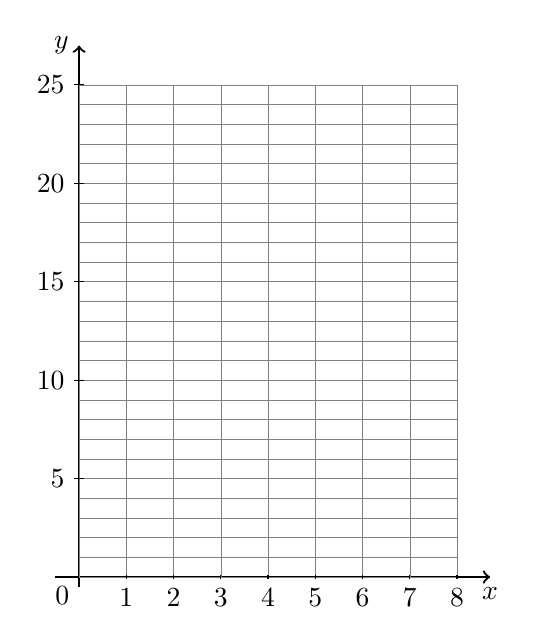
\begin{tikzpicture}[yscale=.25,xscale=.6]
    \draw [->, thick] (0,-.5) -- (0,27) node[left] {$y$};
    \draw [->, thick] (-.5,0) -- (8.7,0) node[below] {$x$};
    \draw[help lines, gray] (0,0) grid (8.01,25.01);
    \foreach \x in {1,...,8} \draw (\x,.1)  -- (\x,-.1)  node[below] {\x};
    \foreach \y in {5,10,...,25} \draw (.1,\y) -- (-.1,\y) node[left] {\y};        
\node[below left] at (0,0) {0};
  \end{tikzpicture}
\end{minipage}
\ifdefined\prof
\clearpage
\fi
\item  \phantom{coisa}

  \begin{minipage}{.4\textwidth}
 \begin{table}[H]
    \setlength\tabcolsep{2.5pt}
\begin{tabu} to .4\textwidth{|c|c|c|}
  \hline
  \thead
  $\bm{[a,b]}$ & $\bm{f(0) = 0}$ & $\bm{\Delta y/\Delta x}$ \\
  \hline
  $[0,1]$ & $f(1) = \phantom{1000} $ & 10 \\
  \hline
  $[1,2]$ & $f(2) = \phantom{1000} $ & -8 \\
  \hline
  $[2,3]$ & $f(3) = \phantom{1000} $ & 6 \\
  \hline
  $[3,4]$ & $f(4) = \phantom{1000} $ & 0 \\  
  \hline
\end{tabu}
\end{table}
\end{minipage}\hfill
\begin{minipage}{.4\textwidth}
  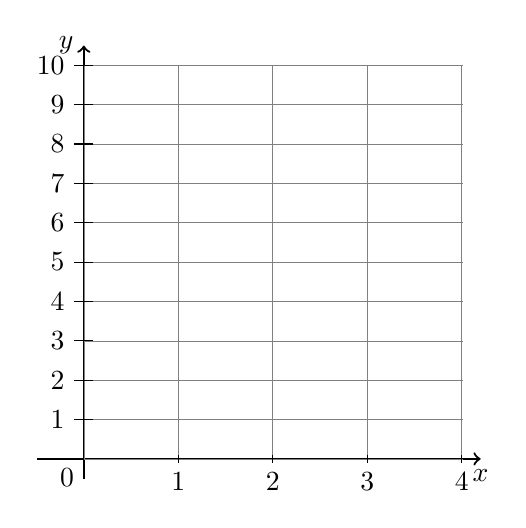
\begin{tikzpicture}[yscale=.5,xscale=1.2]
    \draw [->, thick] (0,-.5) -- (0,10.5) node[left] {$y$};
    \draw [->, thick] (-.5,0) -- (4.2,0) node[below] {$x$};
    \draw[help lines, gray] (0,0) grid (4.01,10.01);
    \foreach \x in {1,...,4} \draw (\x,.1)  -- (\x,-.1)  node[below] {\x};
    \foreach \y in {1,...,10} \draw (.1,\y) -- (-.1,\y) node[left] {\y};        
\node[below left] at (0,0) {0};
  \end{tikzpicture}
  \end{minipage}

  
\item  \phantom{coisa}

  \begin{minipage}{.4\textwidth}
 \begin{table}[H]
    \setlength\tabcolsep{2.5pt}
\begin{tabu} to .4\textwidth{|c|c|c|}
  \hline
  \thead
  $\bm{[a,b]}$ & $\bm{f(0) = 0}$ & $\bm{\Delta y/\Delta x}$ \\
  \hline
  $[0,1]$ & $f(1) = \phantom{1000} $ & 1 \\
  \hline
  $[1,2]$ & $f(2) = \phantom{1000} $ & 3 \\
  \hline
  $[2,3]$ & $f(3) = \phantom{1000} $ & 5 \\
  \hline
  $[3,4]$ & $f(4) =  $\phantom{1000} & 7 \\  
  \hline
  $[4,5]$ & $f(5) =  $ \phantom{1000} & 5 \\  
  \hline
  $[5,6]$ & $f(6) =  $ \phantom{1000}& 3 \\  
  \hline
  $[6,7]$ & $f(7) =  $\phantom{1000} & 1 \\  
  \hline
  $[7,8]$ & $f(8) =  $\phantom{1000} & 0 \\  
  \hline  
\end{tabu}
\end{table}
\end{minipage}\hfill
\begin{minipage}{.4\textwidth}
  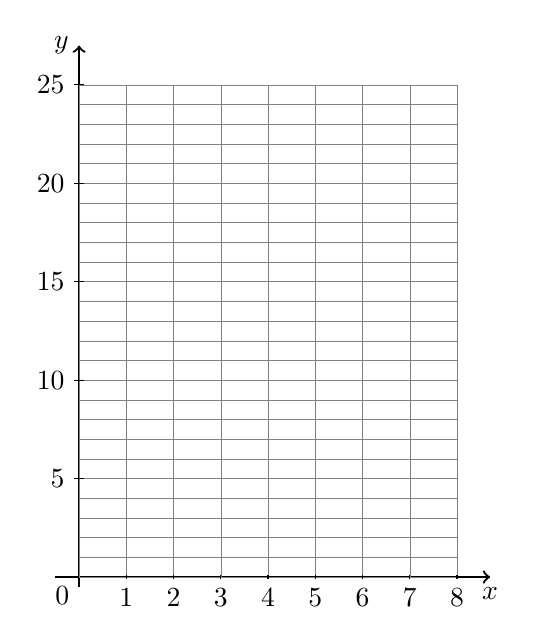
\begin{tikzpicture}[yscale=.25,xscale=.6]
    \draw [->, thick] (0,-.5) -- (0,27) node[left] {$y$};
    \draw [->, thick] (-.5,0) -- (8.7,0) node[below] {$x$};
    \draw[help lines, gray] (0,0) grid (8.01,25.01);
    \foreach \x in {1,...,8} \draw (\x,.1)  -- (\x,-.1)  node[below] {\x};
    \foreach \y in {5,10,...,25} \draw (.1,\y) -- (-.1,\y) node[left] {\y};        
\node[below left] at (0,0) {0};
  \end{tikzpicture}
\end{minipage}
  
\end{enumerate}

\ifdefined\prof
\clearpage
\begin{solucao}
\begin{multicols}{2}


\begin{enumerate}

\tikzstyle{circ}=[fill,circle, inner sep=1.5pt, session3]
\item\adjustbox{valign=t}{
\begin{tikzpicture}[yscale=.5,xscale=1.2, every node/.style={black}, every path/.style={black}]
    \draw [->, thick] (0,-.5) -- (0,11) node[left] {$y$};
    \draw [->, thick] (-.5,0) -- (4.2,0) node[below] {$x$};
    \draw[help lines, gray] (0,0) grid (4.01,10.01);
    \foreach \x in {1,...,4} \draw (\x,.1)  -- (\x,-.1)  node[below] {\x};
    \foreach \y in {1,...,10} \draw (.1,\y) -- (-.1,\y) node[left] {\y};        
\node[below left] at (0,0) {0};
\draw [dashed,session3, thick] (0,1) -- (4,9);
\foreach \x/\y in {0/1,1/3,2/5,3/7,4/9} \node [circ] at (\x,\y) {};
  \end{tikzpicture}}

\item\adjustbox{valign=t}{
\begin{tikzpicture}[yscale=.5,xscale=1.2, every node/.style={black}, every path/.style={black}]
    \draw [->, thick] (0,-.5) -- (0,11) node[left] {$y$};
    \draw [->, thick] (-.5,0) -- (4.2,0) node[below] {$x$};
    \draw[help lines, gray] (0,0) grid (4.01,10.01);
    \foreach \x in {1,...,4} \draw (\x,.1)  -- (\x,-.1)  node[below] {\x};
    \foreach \y in {1,...,10} \draw (.1,\y) -- (-.1,\y) node[left] {\y};        
\node[below left] at (0,0) {0};
\draw [dashed,session3, thick] (0,10) -- (4,2);
\foreach \x/\y in {0/10,.5/9,1/8,1.5/7,2/6,2.5/5,3/4,3.5/3,4/2} \node [circ] at (\x,\y) {};
  \end{tikzpicture}}

\item\adjustbox{valign=t}{
\begin{tikzpicture}[yscale=.25,xscale=.6, every node/.style={black}, every path/.style={black}]
    \draw [->, thick] (0,-.5) -- (0,22) node[left] {$y$};
    \draw [->, thick] (-.5,0) -- (8.7,0) node[below] {$x$};
    \draw[help lines, gray] (0,0) grid (8.01,21);
    \foreach \x in {1,...,8} \draw (\x,.1)  -- (\x,-.1)  node[below] {\x};
    \foreach \y in {5,10,...,20} \draw (.1,\y) -- (-.1,\y) node[left] {\y};        
\node[below left] at (0,0) {0};
\draw [dashed,session3, thick] (0,0) -- (2,2) -- (4,6) -- (6,12) -- (8,20);
\foreach \x/\y in {0/0,2/2,4/6,6/12,8/20} \node [circ] at (\x,\y) {};
  \end{tikzpicture}}

\item\adjustbox{valign=t}{
\begin{tikzpicture}[yscale=.5,xscale=1.2, every node/.style={black}, every path/.style={black}]
    \draw [->, thick] (0,-.5) -- (0,11) node[left] {$y$};
    \draw [->, thick] (-.5,0) -- (4.2,0) node[below] {$x$};
    \draw[help lines, gray] (0,0) grid (4.01,10.01);
    \foreach \x in {1,...,4} \draw (\x,.1)  -- (\x,-.1)  node[below] {\x};
    \foreach \y in {1,...,10} \draw (.1,\y) -- (-.1,\y) node[left] {\y};        
\node[below left] at (0,0) {0};
\draw [dashed,session3, thick] (0,0) -- (1,10) -- (2,2) -- (3,8) -- (4,8);
\foreach \x/\y in {0/0,1/10,2/2,3/8,4/8} \node [circ] at (\x,\y) {};
  \end{tikzpicture}}

\item\adjustbox{valign=t}{
\begin{tikzpicture}[yscale=.25,xscale=.6, every node/.style={black}, every path/.style={black}]
    \draw [->, thick] (0,-.5) -- (0,27) node[left] {$y$};
    \draw [->, thick] (-.5,0) -- (8.7,0) node[below] {$x$};
    \draw[help lines, gray] (0,0) grid (8.01,25.01);
    \foreach \x in {1,...,8} \draw (\x,.1)  -- (\x,-.1)  node[below] {\x};
    \foreach \y in {5,10,...,25} \draw (.1,\y) -- (-.1,\y) node[left] {\y};        
\node[below left] at (0,0) {0};
\draw [dashed,session3, thick] (0,0) -- (1,1) -- (2,4) -- (3,8) -- (4,15) -- (5,20) -- (6,23) -- (7,24) -- (8,24);
\foreach \x/\y in {0/0,1/1,2/4,3/8,4/15,5/20,6/23,7/24,8/24} \node [circ] at (\x,\y) {};
  \end{tikzpicture}}
\end{enumerate}
  \end{multicols}
\end{solucao}
\fi

\end{document}